\message{ !name(hw1.tex)}\documentclass{article}
\usepackage{CJKutf8}
\usepackage{amsmath}
\usepackage{amsfonts}
\usepackage{amsthm}
\usepackage{amssymb}
\usepackage{graphicx}

\title{\textbf{Multi. Stat. HW1}}
\author{赵浩宇 2016012390}
\date{}

\begin{document}

\message{ !name(hw1.tex) !offset(-3) }

\begin{CJK}{UTF8}{gbsn}
  \maketitle
\end{CJK}

\section{Problem 1}
If we let the distribution to be $N(0,1)$, the percentage the the data that lies outside the outside bars is about to be $0.7\%$.
\begin{proof}
  \begin{equation*}
    Q_3  = \Phi^{-1}\left(0.75\right)
        \approx 0.6745
  \end{equation*}
  \begin{equation*}
    Q_1  = -Q_3
         \approx -0.6745
  \end{equation*}
  \begin{equation*}
    IQR  = Q_3 - Q_1
         \approx 1.349
  \end{equation*}
  \begin{align*}
    upper\_outlier  &= Q_3 + 1.5 \cdot IQR\\
                    &= 0.6745 + 1.5 \times 1.349\\
                    &= 2.698\\
                    &\approx 2.7
  \end{align*}
  So the portion that is bigger than the upper outside bar is about
  \begin{equation*}
    1 - \Phi^{-1}\left(2.7\right) \approx 0.0035
  \end{equation*}
  So the portion that lie outside the outside bars should be about $0.007 \approx 0.7\%$.
\end{proof}
If the data follow the distribution $N(0, \sigma^2)$, then the portion should also be about $0.7\%$.\\
 We can get the data follow the distribution $N(0,\sigma^2)$ by multiplying the standard normal distribution by $\sigma$, and the quantiles, IQR, and the value of the outside bars are also multiplied by $\sigma$. The data follows $N(0,\sigma^2)$ that lies outside the outside bars also lies outside the outisde bars (of the dist. $N(0,1)$) when it is devided by $\sigma$, so the percentage of data that lies outside the outside bars in this problem is the same as the previous problem.
\clearpage


\section{Problem 2}
\textbf{a.}\\
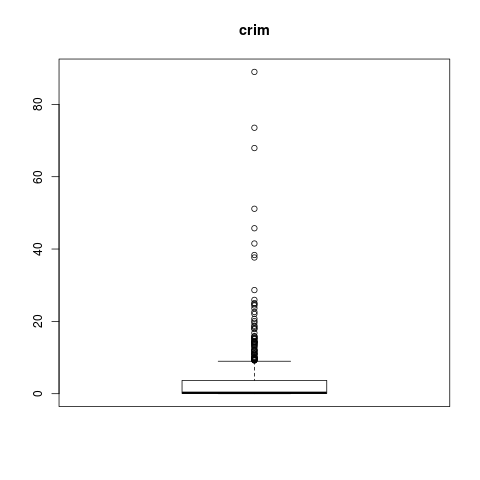
\includegraphics[width=3in]{1.png}
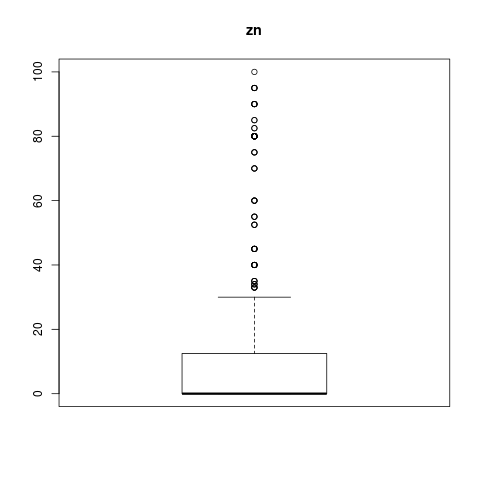
\includegraphics[width=3in]{2.png}
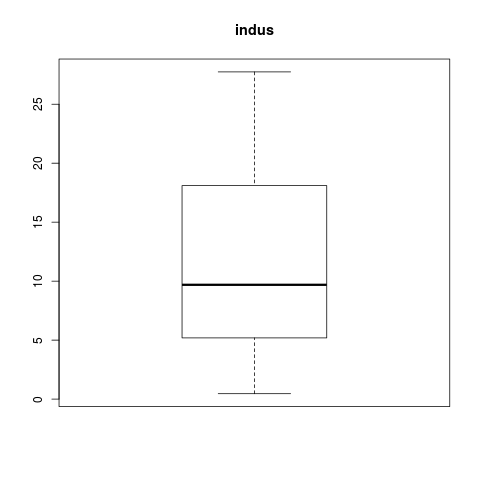
\includegraphics[width=3in]{3.png}
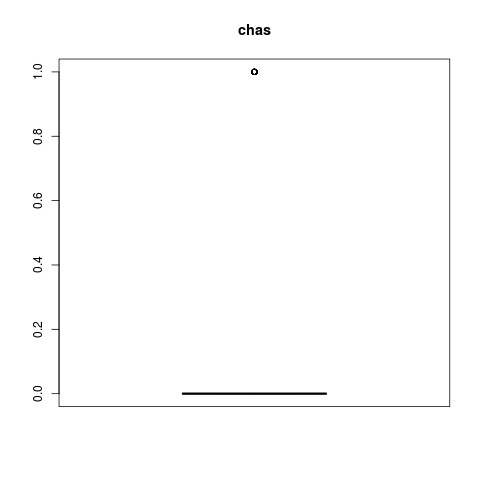
\includegraphics[width=3in]{4.png}
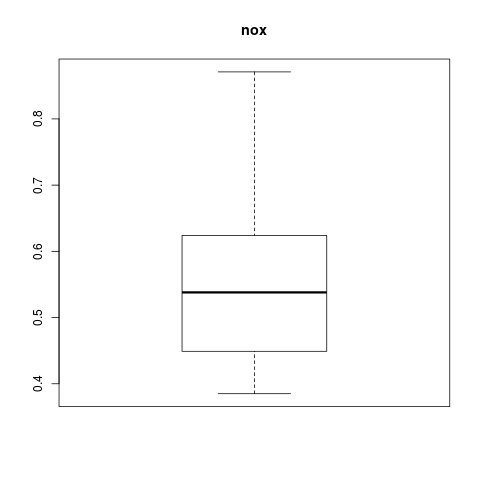
\includegraphics[width=3in]{5.png}
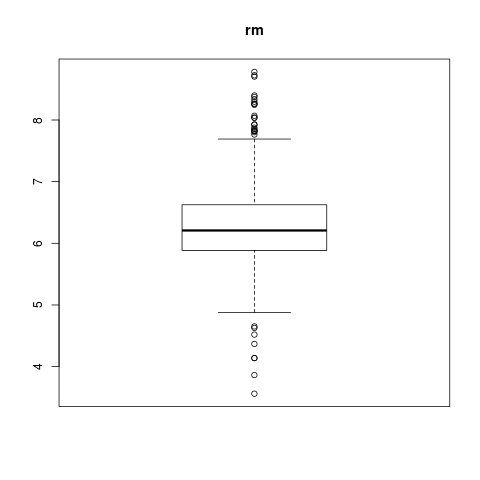
\includegraphics[width=3in]{6.png}
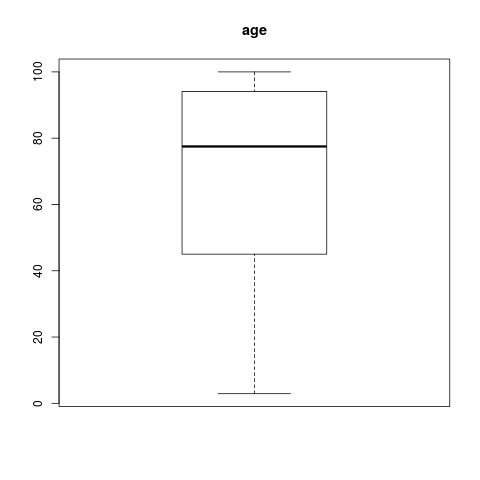
\includegraphics[width=3in]{7.png}
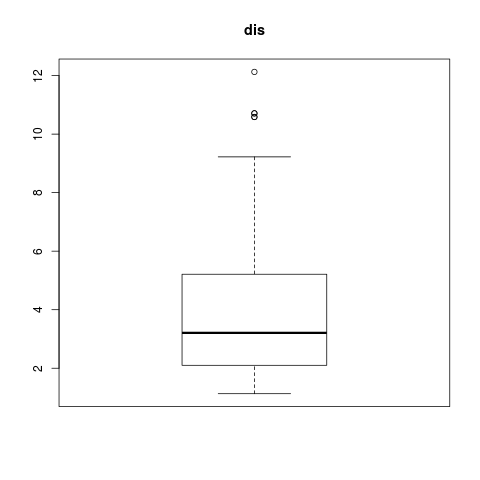
\includegraphics[width=3in]{8.png}
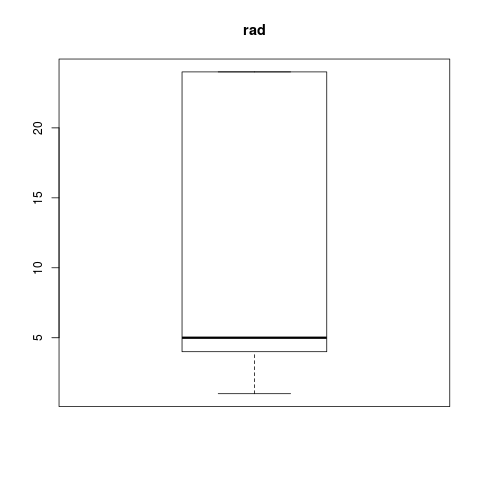
\includegraphics[width=3in]{9.png}
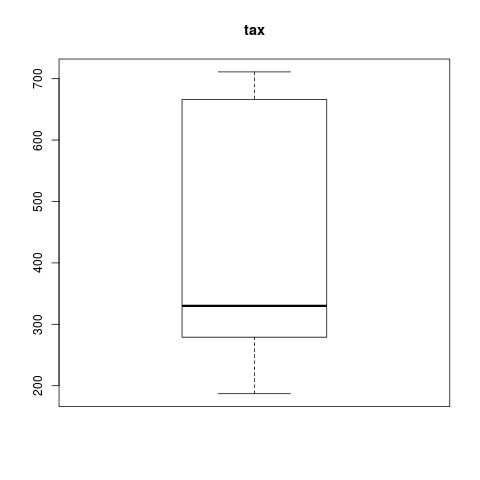
\includegraphics[width=3in]{10.png}
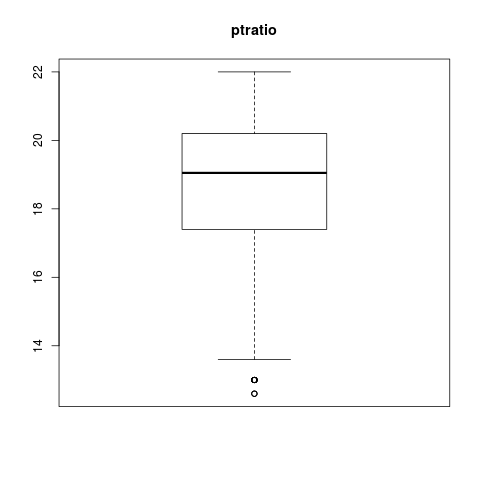
\includegraphics[width=3in]{11.png}
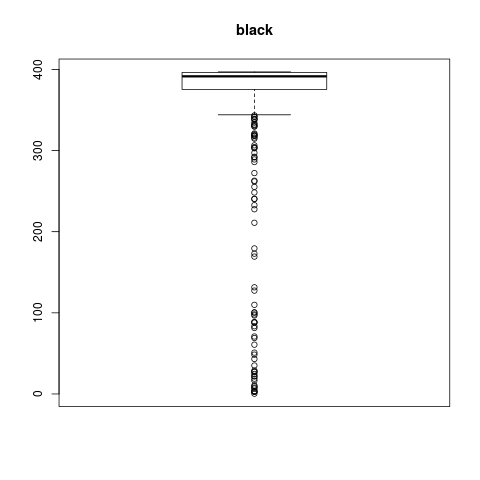
\includegraphics[width=3in]{12.png}
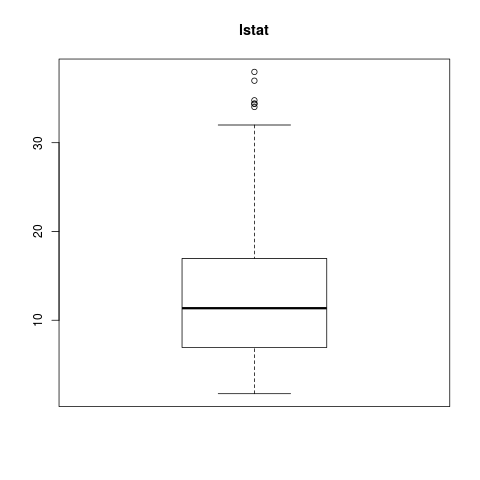
\includegraphics[width=3in]{13.png}
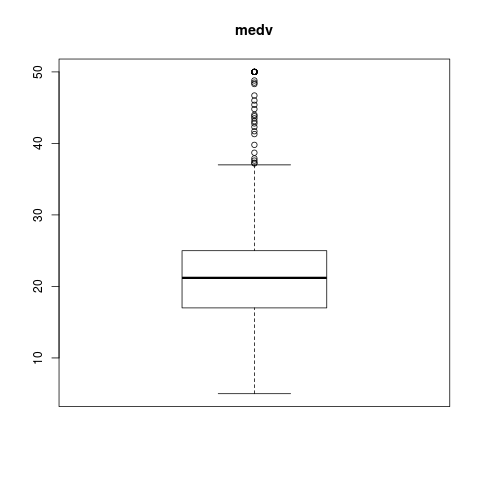
\includegraphics[width=3in]{14.png}
~\\
\clearpage
\textbf{b.}\\
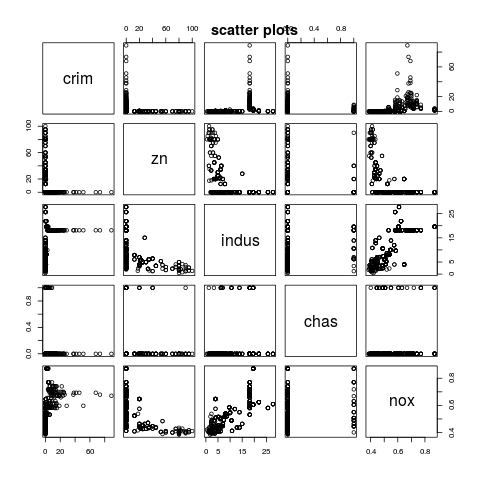
\includegraphics[width=6in]{scatter.png}
~\\
The figure above is the matrix scatter plots for the first five variables.\\
~\\
\clearpage
\textbf{c.}\\
The correlation matrix with 4 digits is showned below.\\
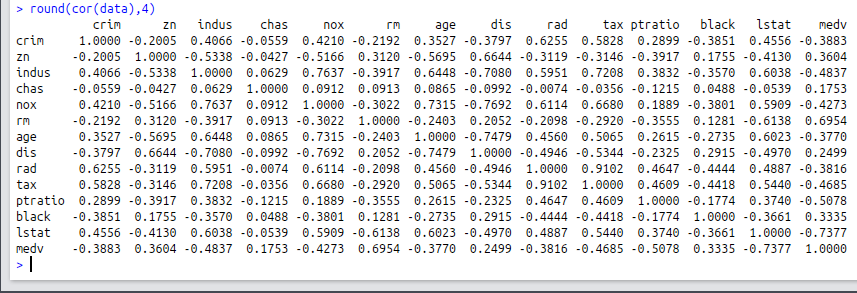
\includegraphics[width=6in]{corre.png}
~\\


\section{Problem 3}
\begin{proof}
\begin{equation*}
  r_{xy} = \frac{1}{n}\frac{\sum_{i=1}^n \left(x_i - \overline{x}\right)\left(y_i - \overline{y}\right)}{s_x \cdot s_y}
\end{equation*}
According to the conditions, the data was changed linearly, we can get:
\begin{align*}
  s_i &= ax_i + b\\
  t_i &= cy_i + d\\
  \overline{s} &= a\overline{x} + b\\
  \overline{t} &= c\overline{y} + d\\
  s_s &= as_x\\
  s_t &= cs_y\\
\end{align*}
Then we can get:
\begin{align*}
  r_{st} &= \frac{\sum_{i=1}^n \left(s_i - \overline{s}\right)\left(t_i - \overline{t}\right)}{n \cdot s_s \cdot s_t}\\
  &= \frac{\sum_{i=1}^n \left(ax_i + b - a\overline{x} - b\right)\left(cy_i + d - c\overline{y} - d\right)}{n \cdot a \cdot s_x \cdot c \cdot s_y}\\
  &=\frac{1}{n}\frac{\sum_{i=1}^n a \cdot \left(x_i - \overline{x}\right) \cdot c \cdot \left(y_i - \overline{y}\right)}{a\cdot s_x \cdot c \cdot s_y}\\
  &=\frac{1}{n}\frac{\sum_{i=1}^n \left(x_i - \overline{x}\right)\left(y_i - \overline{y}\right)}{s_x \cdot s_y}\\
  &=r_{xy}
\end{align*}
So the linear transformation does not change the sample correlation.
\end{proof}


\section*{Problem 4}
\subsection*{2.8}
The characteristic polynomial of the matrix is
\begin{equation*}
  f(\lambda) = (1-\lambda)(-2-\lambda) - 2^2.
\end{equation*}
Set $f(\lambda) = 0$ and we can get the root of $f(\lambda)$,
\begin{equation*}
  \lambda_1 = 2, \lambda_2 = -3.
\end{equation*}
Let
\begin{equation*}
  \mathbf{e}_1 = \left[
    \begin{matrix}
      \frac{2}{\sqrt{5}}\\
      \frac{1}{\sqrt{5}}
    \end{matrix}\right],
  \mathbf{e}_2 = \left[
    \begin{matrix}
      \frac{1}{\sqrt{5}}\\
      -\frac{2}{\sqrt{5}}
    \end{matrix}\right]
\end{equation*}
We can see that
\begin{equation*}
  \mathbf{Ae}_1 = \lambda_1\mathbf{e}_1, \mathbf{Ae}_2 = \lambda_2\mathbf{e}_2, \lVert \mathbf{e}_1 \rVert = \lVert \mathbf{e}_2 \Vert = 1,
\end{equation*}
So $\mathbf{e}_1$ and $\mathbf{e}_2$ are 2 normalized eigenvectors of $\mathbf{A}$.
And according to the sqectual theorem,
\begin{equation*}
  A = \lambda_1\mathbf{e}_1\mathbf{e}_1^T + \lambda_2\mathbf{e}_2\mathbf{e}_2^T = 2\left[
    \begin{matrix}
      \frac{2}{\sqrt{5}}\\
      -\frac{1}{\sqrt{5}}
    \end{matrix}\right]\left[\frac{2}{\sqrt{5}}, \frac{1}{\sqrt{5}}\right] - 3\left[
    \begin{matrix}
      \frac{1}{\sqrt{5}}\\
      -\frac{2}{\sqrt{5}}
    \end{matrix}\right]\left[\frac{1}{\sqrt{5}} - \frac{2}{\sqrt{5}}\right].
\end{equation*}

\subsection*{2.9}
\textbf{a.}\\
\begin{equation*}
  B = \left[
    \begin{matrix}
      \frac{1}{3}&\frac{1}{3}\\
      \frac{1}{3}&-\frac{1}{6}
    \end{matrix}\right]
\end{equation*}
Then we can find that $AB = BA = I$, so $A_{-1} = B$.\\
\textbf{b.}\\
\begin{equation*}
  S = \left[\mathbf{e}_1, \mathbf{e}_2\right], \Sigma = \left[
    \begin{matrix}
      2&0\\
      0&-3
    \end{matrix}\right], \Sigma^{-1} = \left[
    \begin{matrix}
      \frac{1}{2}&0\\
      0&-\frac{1}{3}
    \end{matrix}\right].
\end{equation*}
Then we have $A = S\Sigma S^{-1}$.
Because $S\Sigma S^{-1} S\Sigma^{-1}S^{-1} = S\Sigma\Sigma^{-1}S^{-1} = I$,
we can know that $A^{-1} = S\Sigma^{-1}S^{-1}$, so the eigenvalues of $A^{-1}$ is,
\begin{equation*}
  \mu_1 = \frac{1}{2}, \mu_2 = -\frac{1}{3}.
\end{equation*}
And the normalized eigenvectors remain the same as the eigenvectors of $A$, so
\begin{equation*}
  \mathbf{v}_1 = 
\end{equation*}
\textbf{c.}\\

\subsection*{2.15}
The quadratic form
\begin{equation*}
  \mathbf{Q} = \mathbf{x}^T\mathbf{Ax}, \mathbf{x}^T = \left[x_1, x_2\right], \mathbf{A} = \left[
        \begin{matrix}
          3&-1\\
          -1&3
        \end{matrix}\right]
\end{equation*}
We can compute the eigenvalues of $\mathbf{A}$,
\begin{equation*}
  \lambda_1 = 4, \lambda_2 = 2.
\end{equation*}
So it's positive definite.

\end{document}
\message{ !name(hw1.tex) !offset(-200) }
